\chapter{Proposed improvements and results}
\label{cha:improvements}

In this chapter, we will present some \textbf{improvements} to live streaming protocols and libraries that we believe produce a \textbf{better overall quality of experience} in video streaming. The proposed improvements are based on the findings presented in the previous chapter.

Specifically, we will first dive into the adaptation algorithms of \dashjs{} to assess that the default configuration is not suitable for low-latency live streaming. Then, we will propose a better configuration which also involves writing a custom ABR rule.

We will then look at how we can take advantage of HTTP/3 features, such as priorities and stream resetting, to implement a new live streaming approach where video playback stalls are avoided if the video buffer is temporarily empty. We will do so with a combination of HTTP prioritization and on-the-fly generation of filler segments on the client side, thanks to WebCodecs API and WebAssembly. For this part, we will modify the \hlsjs{} library.

Finally, we will show how the proposed solution produces fewer playback stalls and avoids the increase of live latency in the case of network congestion, with an overall smoother live streaming user experience.

\section{\dashjs{} bitrate adaptation algorithm improvements}
\label{sec:improvements/dashjs}

In Section \ref{sec:eval/abr/dashjs} we have shown how in some cases the default configuration of \dashjs{} makes the video quality oscillate too frequently with a low-latency live stream. Specifically, Figure \ref{fig:eval_abr_dashjs} represents the buffer health plot, where we can see that in the second half of the experiment the media bitrate chosen by \dashjs{} frequently changes and most of the time stays at a lower value than it should, even if the network bandwidth is consistently above 8 Mbps.

The decision on which bitrate should be requested next is the task of the \textbf{rate adaptation algorithm}, which every library typically implements differently. There are in fact many approaches to solving the problem and there is no clear consensus on which is the best.

The core idea of adaptation algorithms is to choose the best quality level so that the bitrate is lower than the available network bandwidth. There are two main approaches to make this decision:

\begin{itemize}
    \item \textbf{Throughput-based}: the most intuitive approach, consisting of continuously calculating an estimate of the network bandwidth and then selecting the highest bitrate in the ladder which is lower than the bandwidth estimate.
    \item \textbf{Buffer-based}: an alternative approach that observes the occupancy of the buffer to determine whether the decision to increase/dicrease the bitrate should be made. This approach avoids the need to keep a bandwidth estimate.
\end{itemize}

\dashjs{} uses a combination of these two approaches with a strategy called \texttt{DYNAMIC}, which was first introduced in \cite{dashjs_dynamic}. The \texttt{DYNAMIC} strategy switches between a throughput-based approach, named \texttt{THROUGHPUT}, and a buffer-based approach, \texttt{BOLA}.\cite{bola} The idea of switching between the two is based on the fact that each algorithm works best in different situations. In particular, the throughput-based algorithm performs better when the buffer is low or empty, while \texttt{BOLA} (buffer-based) performs better when the buffer level is sufficiently large.

The algorithm that switches between \texttt{THROUGHPUT} and \texttt{BOLA} is therefore based on a threshold that is applied on the buffer level (for each media track). The following code snippet taken from the \dashjs{} source code (\texttt{AbrController} class) shows how the decision on whether to use \texttt{BOLA} is made:

\begin{minted}[frame=single,linenos,breaklines,highlightlines=2]{js}
const useBufferABR = isUsingBufferOccupancyAbrDict[mediaType];
const newUseBufferABR = bufferLevel > (useBufferABR ? switchOffThreshold : switchOnThreshold);
isUsingBufferOccupancyAbrDict[mediaType] = newUseBufferABR;

if (newUseBufferABR !== useBufferABR) {
    if (newUseBufferABR) {
        logger.info('[' + mediaType + '] switching from throughput to buffer occupancy ABR rule');
    } else {
        logger.info('[' + mediaType + '] switching from buffer occupancy to throughput ABR rule');
    }
}
\end{minted}

The relevant part is line 2, where the new decision on whether buffer-based ABR should be used is made based on whether the current buffer level (in seconds) is greater than a threshold.

The \texttt{switchOffThreshold}/\texttt{switchOnThreshold} are calculated from the value of a property called \texttt{stableBufferTime}. Basically, when the buffer level exceeds a threshold value that is considered stable, the \texttt{DYNAMIC} algorithm switches to the buffer-based approach (\texttt{BOLA}), while going back to \texttt{THROUGHPUT} when the buffer level is less than half of the \texttt{stableBufferTime}.

\begin{minted}[frame=single]{js}
const switchOnThreshold = stableBufferTime;
const switchOffThreshold = 0.5 * stableBufferTime;
\end{minted}

The aim is to avoid continuous oscillations between the two strategies, although this does not work well in practice according to our tests. In fact, in the case of a live stream, \texttt{stableBufferTime} is assigned to the live delay target (the configuration parameter we introduced in Section \ref{sec:testbed/frontend/dashjs}). So, for example, if the live delay is 4 seconds, this means that the \texttt{DYNAMIC} algorithm will switch from \texttt{THROUGHPUT} to \texttt{BOLA} when the buffer level goes above 4 seconds, and will switch back to \texttt{THROUGHPUT} when the buffer level goes below 2 seconds.

The problem is that with such a low target live latency, the buffer level tends to oscillate quite a lot and often goes below the threshold of 2 seconds, as can be seen in Figure \ref{fig:eval_abr_dashjs} as an example. In practice, this means that the default \texttt{DYNAMIC} ABR strategy of \dashjs{} will switch between the two approaches very often. This behavior is probably undesirable, as it does not leave time for the algorithm to make proper decisions.

This behavior is also in contrast with the threshold used by the paper that introduced the \texttt{DYNAMIC} strategy and tested its performance. In fact, in \cite{dashjs_dynamic} the threshold value is fixed at 10 seconds. Therefore, following the recommendation of \cite{dashjs_dynamic} for low-latency streams we decided to disable the \texttt{DYNAMIC} strategy and force the \texttt{THROUGHPUT} one. This can be done in \dashjs{} through the settings:

\begin{minted}[frame=single]{js}
player.updateSettings({
    streaming: {
        abr: {
            ABRStrategy: 'abrThroughput'
        }
    }
});
\end{minted}

While we were looking at the internals of \dashjs{} to investigate the issue with \texttt{DYNAMIC}, we discovered that the library includes support for \textbf{additional ABR rules} that should help in cases when the ABR strategy is not enough to make proper decisions about the next bitrate. These rules are by default:

\begin{itemize}
    \item \texttt{DroppedFramesRule}: measures the dropped frames during playback. If they exceed 15\%, the rule switches to a lower bitrate.
    \item \texttt{SwitchHistoryRule}: observes the switch history and avoids switches to higher bitrates that caused quality drops in the past, according to the switch history.
    \item \texttt{AbandonRequestsRule}: calculates whether the loading of a segment should be canceled because it is estimated that it will not be loaded in time for playback, only if there is a lower bitrate that could instead be loaded in the remaining time. This rule acts as an emergency switch down.
    \item \texttt{InsufficientBufferRule}: this rule puts an upper limit on the bitrate, depending on the current buffer health.
\end{itemize}

In particular, the \texttt{InsufficientBufferRule} was found to be the most aggressive in lowering the bitrate even when it was not needed. This happens because it bases the decision on the buffer level, which, as we have seen, is always quite small in a low-latency scenario. More in detail, the \texttt{InsufficientBufferRule} listens to the \texttt{BUFFER\_EMPTY} event and requests a switch to the minimum bitrate when that happens. Otherwise, the rule calculates the maximum bitrate (to be used as the limit) depending on the throughput, so that a whole segment can be downloaded before the buffer runs out. The relevant lines of the rule that perform this computation are the following:

\begin{minted}[frame=single,linenos,breaklines,highlightlines=4]{js}
const throughput = throughputHistory.getAverageThroughput(mediaType, isDynamic);
const bufferLevel = dashMetrics.getCurrentBufferLevel(mediaType);
const fragmentDuration = representationInfo.fragmentDuration;
const bitrate = throughput * (bufferLevel / fragmentDuration) * INSUFFICIENT_BUFFER_SAFETY_FACTOR;
\end{minted}

Line 4 is where the upper limit is calculated. Since \texttt{(bufferLevel / fragmentDuration)} can be seen as the number/fraction of segments currently in the buffer, the maximum bitrate is calculated as a multiplication between the current throughput estimate and the number of segments in the buffer. However, there is a safety factor of 0.5 that effectively halves the maximum bitrate. When the bandwidth estimate is conservative (or has still to adapt to the new network conditions) or the buffer level is kept low on purpose to achieve lower latency, this rule tends to limit the video bitrate too aggressively.

For these reasons, we decided to disable the \texttt{InsufficientBufferRule} and instead create a \textbf{custom rule} that acts only when the buffer is actually empty. In this way, we avoid overreactions of the algorithm deriving from the low latency. The rule can be disabled as follows:

\begin{minted}[frame=single]{js}
player.updateSettings({
    streaming: {
        abr: {
            ABRStrategy: 'abrThroughput'
            additionalAbrRules: {
                insufficientBufferRule: false
            }
        }
    }
});
\end{minted}

The new custom rule can instead be added using the method shown in the following line, without having to modify and rebuild the library.

\begin{minted}[frame=single]{js}
player.addABRCustomRule('qualitySwitchRules', 'BufferEmptyRule', BufferEmptyRule);
\end{minted}

The implementation of the new \texttt{BufferEmptyRule} is similar to the original, but removes the maximum bitrate cap. Instead, it only forces a switch to the minimum bitrate when the buffer is empty. The following (simplified) code block shows how the check is performed.

\begin{minted}[frame=single,breaklines]{js}
if (currentBufferState.state === MetricsConstants.BUFFER_EMPTY) {
    logger.warning('[' + mediaType + '] BufferEmptyRule: switch to index 0.');
    switchRequest.quality = 0;
    switchRequest.reason = 'BufferEmptyRule: Buffer is empty';
}
\end{minted}

This tweaked configuration, consisting in forcing the \texttt{THROUGHPUT} strategy and modifying the additional rules, produces different results compared to previous experiments. For example, the experiment with the \texttt{lte} dataset no longer shows the issue of oscillating bitrate, as shown in Figure \ref{fig:improvements_dashjs}.

\begin{figure}[h]
    \centering
    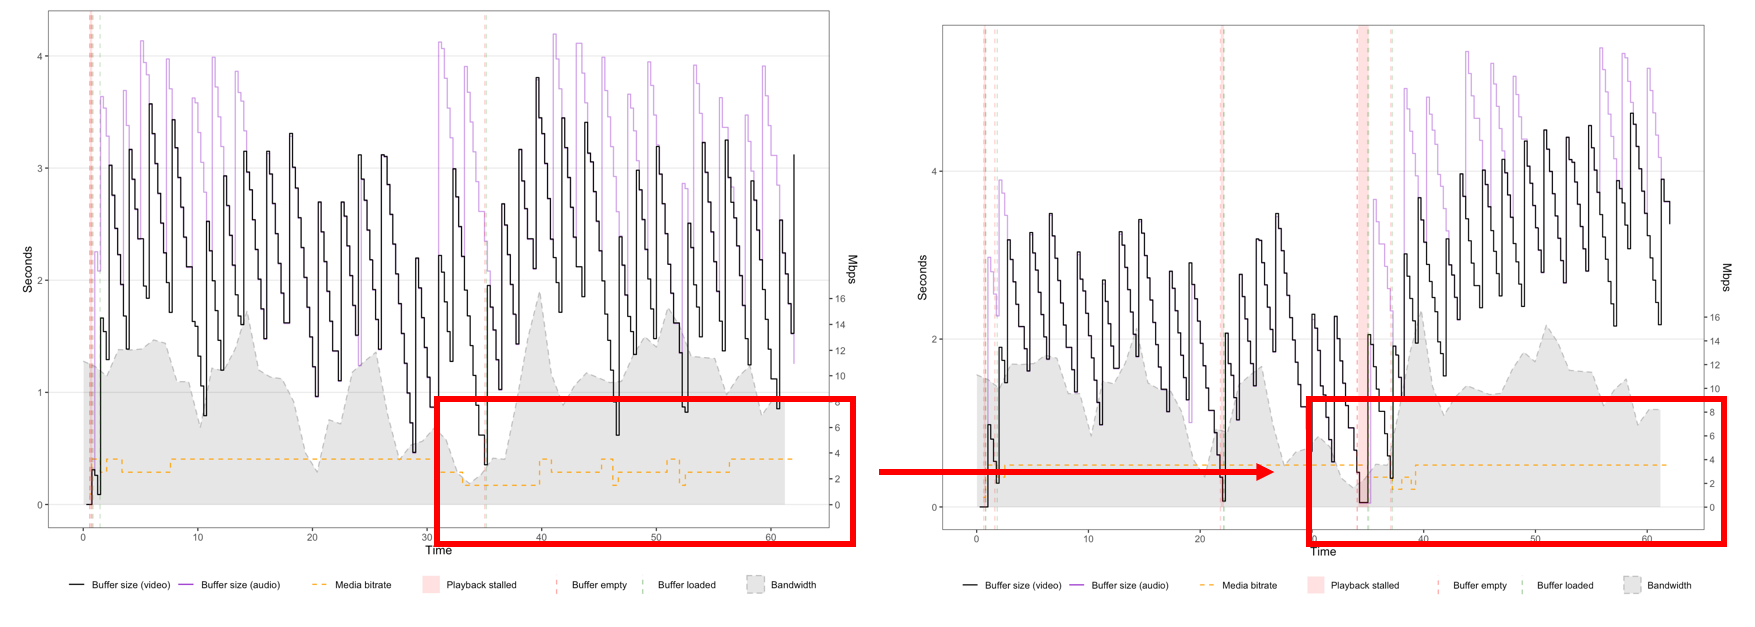
\includegraphics[width=\textwidth]{res/impr_dashjs.png}
    \caption{Buffer health plots showing the difference between the default \dashjs{} ABR configuration and the tweaked configuration.}
    \label{fig:improvements_dashjs}
\end{figure}

\section{Switching to \hlsjs{}}
\label{sec:improvements/hlsjs}

During the development of these improvements to  \dashjs{}, we had the opportunity to take a deeper look at the internals and architecture of \dashjs{}. Unfortunately, we have found that most parts of the code are poorly documented and sometimes do not even have proper TypeScript types definitions. Also, our impression was that it was harder to understand how to extend the library and add new components. One of the reasons is that the library is using plain JavaScript, making it harder to have proper IDE support and type safety.

This led us to switch to \hlsjs{} for the rest of our work. Unlike \dashjs{}, \hlsjs{} is written in TypeScript and is generally better documented. For example, the general architecture and design of the library is explained in detail in the official documentation.\footnote{\url{https://github.com/video-dev/hls.js/blob/master/docs/design.md}}

Unlike \dashjs{}, \hlsjs{} does not use a hybrid approach for the adaptation algorithm. Instead, it uses a standard \textbf{Exponential Weighted Moving Average} (EWMA) bandwidth estimator, which tracks bandwidth samples to produce an estimate of the available network bandwidth. This approach is used for both on-demand and live content, although with different configuration parameters for the EWMA computation.

In addition to the bandwidth estimate, \hlsjs{} also has an \textbf{abandon rule} similar to the one of \dashjs{}. This rule is implemented in the \texttt{\_abandonRulesCheck} method of the \texttt{AbrController} class and is periodically called by a timer. The method calculates the download rate of the current segment and estimates whether the segment will be loaded quickly enough to prevent buffer underflow, based on the estimate of bandwidth. If necessary, the rule will then find a quality level whose bitrate allows the segment to be loaded before buffer starvation, with a safety factor of 80\%. If no level matches this condition, the lower bitrate is chosen.

While we were inspecting the source code that makes the request abandoning feature possible, we found a bug that prevented the check from running in some cases. We therefore reported the issue to the \hlsjs{} developers and a fix is scheduled to be released in early 2023 among other improvements, to the abandon logic.\footnote{\url{https://github.com/video-dev/hls.js/issues/5094}}

\section{Adding priority}
\label{sec:improvements/priority}

As we have seen in Section \ref{sec:eval/abr/hls}, using HLS with the \texttt{spike} pattern tends to produce playback stalls when the bandwidth abruptly drops. This was evident in Figure \ref{fig:eval_abr_hls}. In this section, we will look at how \textbf{adding priority} to some requests helps reducing the issue.

The easiest way to manipulate how \hlsjs{} sends HTTP requests is to use the \texttt{xhrSetup} or \texttt{fetchSetup} configuration options. They can be used to manipulate how HTTP requests are sent respectively with \texttt{XMLHttpRequest} or the \texttt{fetch} API, depending on how \hlsjs{} is configured. In our case we use the default XHR loader, so we need to use the \texttt{xhrSetup} configuration option.

The \texttt{xhrSetup} option takes a function that is called just before sending the HTTP request. In practice, it allows to override how the request is created. In our case, to set the HTTP/3 priority we need to either set the \texttt{Priority} header or the \texttt{priority} query string parameter. In fact, in Section \ref{sec:eval/browsers/priorities} we introduced a patch to the \texttt{h2o} web server that lets us set the priority with the query string parameter.

Since we are interested in \textbf{giving priority only to the audio segments requests}, we need to distinguish which requests correspond to those segments. Doing so in the \texttt{xhrSetup} function does not give a proper way to distinguish the type of request so we must resort to looking at the format of the URL. Since the chunk files contain the ID of the stream (i.e. audio or video), we can implement priority for audio segments as shown in Figure \ref{fig:hlsjs_xhrsetup}.

\begin{figure}[h]
    \centering
    \begin{minted}[frame=single]{ts}
const hls = new Hls({
    xhrSetup: (xhr, url) => {
        if (url.includes('chunk-stream-0')) {
            url = url + '?priority=1';
        } else {
            url = url + '?priority=2';
        }
        xhr.open('GET', url, true);
    }
});
    \end{minted}
    \caption{TypeScript code showing how to configure the XHR request and specify the priority for audio requests. In this case, we are giving the chunks for stream \texttt{1} an HTTP/3 priority of \texttt{1}, while all the other files have priority \texttt{2} (still higher than the default of \texttt{3}).}
    \label{fig:hlsjs_xhrsetup}
\end{figure}

A better way is to override the \texttt{Hls} \textbf{loader} responsible for sending HTTP requests, to modify the URL of the segment based on its type, as shown in Figure \ref{fig:hlsjs_custom_loader}. This is slightly more complex to implement, but we can still avoid to reimplement the whole loader implementation, taking advantage of inheritance.

\begin{figure}
    \centering
    \begin{minted}[frame=single,breaklines,highlightlines=6]{js}
class CustomLoader extends Hls.DefaultConfig.loader {
    constructor(config: HlsConfig) {
        super(config);
        const load = this.load.bind(this);
        this.load = (context: FragmentLoaderContext, config: LoaderConfiguration, callbacks: LoaderCallbacks<LoaderContext>) => {
            if (context.frag.type === 'audio') {
                context.url += '?priority=1';
            } else {
                context.url += '?priority=2';
            }
            load(context, config, callbacks);
        }
    }
}
\end{minted}
    \caption{TypeScript code showing how a custom fragment loader for \hlsjs{} can be implemented to override the priority for specific HTTP requests.}
    \label{fig:hlsjs_custom_loader}
\end{figure}

An instance of the custom fragment loader can then be passed as an option when creating the \texttt{Hls} instance:

\begin{minted}[frame=single]{ts}
const hls = new Hls({
    fLoader: CustomLoader as FragmentLoaderConstructor,
});
\end{minted}

After testing this configuration that gives priority to audio, we quickly discovered that the results were not what we expected. In particular, there were still playback stalls, and in some cases the audio buffer became empty. However, this should not happen since there is always enough bandwidth to transfer the audio segments, which are very small and require just a few hundreds of kbps of bandwidth.

Looking at the logs of \hlsjs{} in debug mode, we discovered that the audio media playlist took several seconds to load. Without an updated playlist, HLS does not know which segment should be requested next. This is different from DASH, where \texttt{SegmentTemplate} allows the client to generate the URLs of the segments without having to update the manifest (Section \ref{sec:bg/technologies/dash}).

Consequently, if we want to give priority to audio, we also need to give priority to the corresponding media playlist, in addition to the segments. This can be done by overriding the \texttt{pLoader} (playlist loader) or the generic \texttt{loader}. In the second case, the implementation of the \texttt{load} method would be something like the following:

\begin{minted}[frame=single]{ts}
const fragmentContext = context as FragmentLoaderContext;
const playlistContext = context as PlaylistLoaderContext;

if (fragmentContext.frag && fragmentContext.frag.type === 'audio' ||
    playlistContext.url && playlistContext.type === 'audioTrack') {
    context.url += '?priority=1';
} else {
    context.url += '?priority=2';
}
\end{minted}

Figure \ref{fig:improvements_hls_pri} shows how this approach affects the buffer health plot. Compared to Figure \ref{fig:eval_abr_hls}, we see that there are \textbf{fewer playback stalls}, even if the video buffer is often empty. Obviously, there is some unpredictability in these experiments, so different runs might show slightly different behaviors. However, the priority to audio is now assigned consistently and better resembles the behavior of HTTP/2 and HTTP/1.1 as seen earlier (Section \ref{sec:eval/non-abr/http-versions}).

\begin{figure}[h]
    \centering
    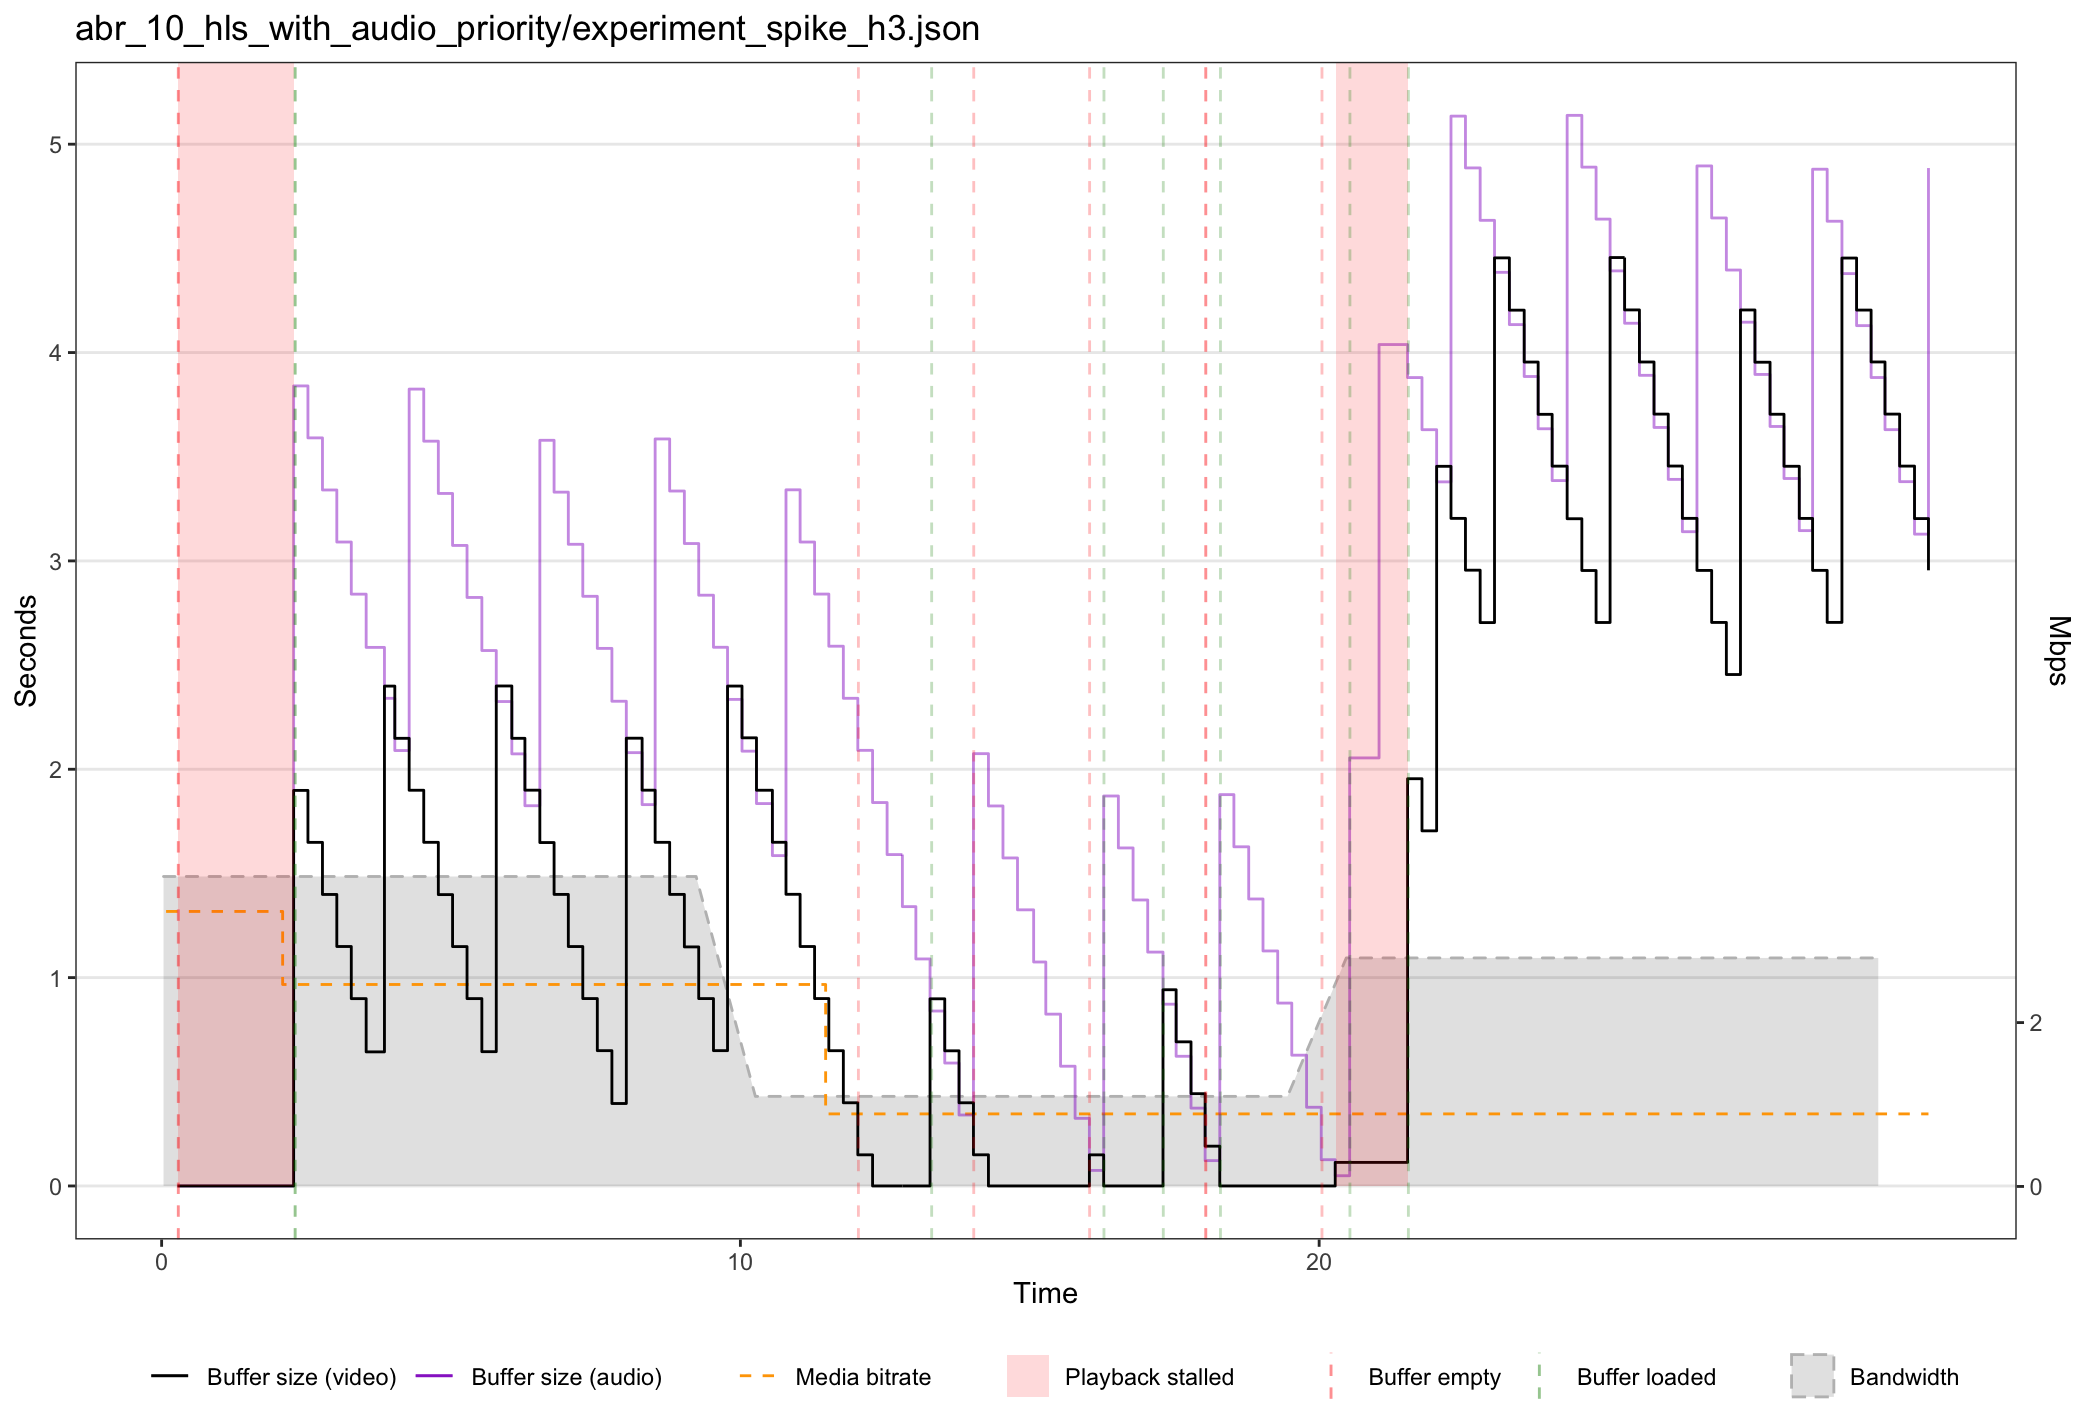
\includegraphics[width=\textwidth]{res/impr_hls_pri.png}
    \caption{Buffer health plot for an HLS experiment with the \texttt{spike} pattern giving priority to the audio.}
    \label{fig:improvements_hls_pri}
\end{figure}

Clearly, when the video buffer is empty the video will appear frozen on screen while the buffer recovers, although the audio will keep playing. Unlike the situation where no priority is specified, \textbf{the live latency of the stream will not increase}.

\section{A new and different live user experience}
\label{sec:improvements/ux}

The behavior that we have shown in the previous section derives from the Chromium implementation of the handling of buffer underflows. This means, for example, that in other browsers when one of the two buffers is empty the playback will immediately stall.

Another limitation is that in Chromium the playback stall is avoided only for three seconds. Ideally, we would like to have more control on how and when this happens, on all browsers.

The final objective is to build \textbf{a user experience with fewer playback stalls}. Usually, when a live stream struggles to adapt to network conditions the viewer is used to see both audio and video stuck for a while during rebuffering. When this happens, latency tends to grow and playback lags behind the edge of the live playlist. As a consequence, users will perceive the action late, possibly by even tens of seconds.

This kind of experience is \textbf{different in comparison to other broadcasting systems}. For example, digital terrestrial and satellite do not have the concept of buffering: if the video signal is not good enough, video and/or audio are temporarily unavailable while the signal recovers, but no latency is introduced, i.e. viewers always see the live action with a fixed delay independently from the signal quality.

Adaptive streaming research has been mostly focused on avoiding empty buffers as much as possible, although in low-latency scenarios entirely avoiding rebuffering is a very hard task. Instead, we can try to implement a solution that tries to resemble the linear TV experience that viewers are already used to. Although subjective, it would likely result in a better Quality of Experience (QoE).

\subsection{Related works}
\label{sec:improvements/ux/related}

There are a few proposals that in the past few years attempted to provide an alternative solution to the problem of video transmission over unreliable networks.

In 2019, the authors of \cite{framediscarding} proposed an approach called \textbf{frame discarding}. The idea was to exploit HTTP/2 streams to transmit each individual video frame independently. When network conditions become adverse, some carefully selected video frames are discarded and their download is aborted through the stream resetting feature of HTTP/2, saving bandwidth and at the same time preserving playback continuity.

In 2021, Facebook presented a draft for \textbf{Reliable (Unreliable) Streaming Protocol} (RUSH), which uses the QUIC protocol to provide a replacement for RTMP for video ingestion on unreliable networks. Video frames are transmitted in independent QUIC streams, providing a way to stop retransmissions if a video frame is not fully delivered on time.\cite{rush}

In 2022, Twitch, the video streaming platform, submitted a draft RFC for \textbf{Warp}, a new protocol for segmented media delivery over QUIC. Warp transmits one video segment per QUIC stream and gives priority to newer video segments and to the audio track. Video segments that cannot be delivered in time are reset at the QUIC stream level to free bandwidth, an approach that Twitch calls \textbf{segment truncation}. Warp can be used for video delivery in the browser thanks to WebTransport, an abstraction of QUIC, although at the time of writing the draft proposal does not include adaptive bitrate support.\cite{warp}

Finally, a new IETF working group, \textbf{Media Over QUIC}, is evaluating how to consolidate video streaming protocols that work over QUIC in a single standardized solution.\footnote{https://datatracker.ietf.org/wg/moq/about/}

\section{Implementation}
\label{sec:improvements/impl}

To our knowledge, the solutions mentioned in Section \ref{sec:improvements/ux/related} are the only attempts that have been publicly proposed to tackle the issue of video streaming from a different perspective.

In this work, we make an attempt to implement an approach similar to the one proposed by Warp, but over HTTP and using an existing ABR protocol. Specifically, we modify the \hlsjs{} library and take advantage of new HTTP features made available by HTTP/3, something that has not been tried before, to our knowledge.

In practice, implementing the solution means tackling the following points:

\begin{itemize}
    \item \textbf{Prioritization of requests}: as we have already seen in depth, audio segments and playlists should be prioritized over video.
    \item \textbf{Segment dropping}: when it is too late for a video segment to be useful, we can cancel its download to free bandwidth.
    \item \textbf{Filler segments}: when a segment is dropped, we need to provide a filler or placeholder to the source buffer. This "fake" segment should be generated on the client side in the browser.
\end{itemize}

\subsection{Segment dropping}
\label{sec:improvements/impl/dropping}

In a live stream, when a video segment has no chance of being loaded in time for playback, we can decide that there is no point in continuing the download and instead discard it. In this way, we free bandwidth that can be used to load the next segment.

In HTTP/3, this can be done by aborting the HTTP request, an action that in practice resets the underlying QUIC stream. Resetting a stream means sending a frame of type \texttt{RESET\_STREAM} and immediately closing the stream, also stopping the transmission of the data, if any.

In \hlsjs{}, video segments are downloaded sequentially, one at a time. Therefore, we can always look at the current segment and estimate whether the segment will not arrive on time and cancel the download if needed. This is somewhat similar to what the \texttt{\_abandonRulesCheck} does, which we mentioned in Section \ref{sec:improvements/hlsjs}. The \texttt{\_abandonRulesCheck} method is called by a JavaScript interval every 100 milliseconds and evaluates whether the current segment is taking too long to load. If so, it will abort the load of the segment.

For our scenario, we needed to implement something similar. As a first attempt, we implemented a simpler mechanism that checks whether we are about to reach the end of the video buffer. We therefore modified the \hlsjs{} source code and specifically the \texttt{AbrController}. We added a new periodic timer for a function named \texttt{fillerCheck}, which calculates how much time is left in the buffer, as shown in the following code block.

\begin{minted}[frame=single]{ts}
const bufferInfo = BufferHelper.bufferInfo(
    media,
    media.currentTime,
    config.maxBufferHole
);

const bufferLength = bufferInfo.len;
const nextFragmentOffset = frag.start - bufferInfo.end;
\end{minted}

The \texttt{bufferLength} variable is self-explanatory: it corresponds to the seconds of media data currently in the buffer between the current video timestamp and the end of the buffer. Obviously, if no data is appended to the buffer the length will decrease at every tick of the timer. The \texttt{nextFragmentOffset} is the time difference between the end of the buffer and the start of the fragment. This is used to understand whether the fragment currently being loaded is actually the one immediately following the end of the buffer. Ideally, the difference should be zero, but timestamps are not always that precise so we use a small tolerance (\texttt{maxBufferHole}).

When the above condition is met and the \texttt{bufferLength} is less than a threshold, we make the decision to abort the segment load. The threshold is set by default to 200 milliseconds (considering the fact that the tick interval is 100 milliseconds), but it is configurable. Another thing that the implementation needs to consider and handle is that the segment loading might be aborted by other rules, for example the \texttt{\_abandonRulesCheck}.

Upon making the decision to abort the segment loading, we cancel the actual download of the segment file. Since we are in the \texttt{AbrController} and have access to the \texttt{Fragment} being loaded, we can directly interact with the \texttt{Loader} instance through the \texttt{loader} property. We therefore modified the \texttt{Loader} interface and defined a new method that mainly performs two operations:

\begin{itemize}
    \item Cancel the HTTP request, and thus reset the underlying QUIC stream in the case of HTTP/3.
    \item Emit an event so that other actions can take place, as we will see in the next section.
\end{itemize}

\subsection{Generating the filler segment}
\label{sec:improvements/impl/filler}

When the segment dropping code makes the decision to discard a video segment and interrupt its loading, the buffer must still be filled with some placeholder data in order not to interrupt playback. We call this "fake" segment a \textbf{filler segment}.

To reproduce the Chromium underflow behavior, which consists of showing the last rendered frame on the video player while the playback continues with audio, we would need to \textbf{generate a video segment on the fly in the browser}. In practice, this means encoding a 2-second video fragment containing a still picture, corresponding to the video frame.

As a first implementation to confirm the feasibility of the solution, we implemented a simpler solution that uses an empty frame with a solid color background. Since H.264 does not necessarily contain timing data, in this way the segment can be generated statically beforehand and reused multiple times. It can even be hardcoded in the client code.

However, the H.264 bitstream alone is not enough to play the segment. In fact, the Media Source Extensions API expects media data to be muxed in the fragmented MP4 format. Consequently, the H.264 data must be inserted into the MP4 container with the correct timing information.

Moreover, since the filler segment is generated with different encoding parameters with respect to the main stream, there is a discontinuity that the video decoder must be aware of. In \texttt{fMP4}, this signaling of the new parameters is done through initialization segments, that is, segments that contain at least the \texttt{ftyp} and \texttt{moov} boxes. This information is shared by all the segments following the init segment, until a new one is found.

Once both the init segment and the segment data are available, they are appended to the \texttt{SourceBuffer} so that the video segment can be played.

\subsection{Muxing in the browser}
\label{sec:improvements/impl/muxing}

As mentioned above, once we have the H.264 bitstream of the video frame we have to \textbf{mux it into the \texttt{fMP4} container} to produce the segment. The segment does not need to contain 25 frames per second, but it can actually contain only one video frame with a duration of 2 seconds (and the correct start timestamp).

The browser APIs do not provide a way to mux or transmux video data, therefore we had to rely on other libraries. An important fact that affects the implementation is that we are dealing with the fragmented MP4 container format and not simply MP4. In fact, not all libraries support the \texttt{fMP4} format.

After investigating several possible options, we came to the conclusion that there was no complete JavaScript library that implements \texttt{fMP4} muxing in the browser. In fact, \texttt{fMP4} muxing is usually performed directly by the libraries that use the MSE API, such as \hlsjs{} when transmuxing from MPEG-2 TS to \texttt{fMP4}.

Instead of delving into a manual JavaScript implementation of \texttt{fMP4} fragments muxing from the raw H.264 bitstream, we decided to experiment with an approach based on \texttt{WebAssembly}, which turned out to be successful.

\texttt{WebAssembly} (WASM) is a low-level binary format that can be used as a build target of many programming languages. It is meant to provide an efficient alternative to JavaScript: a WASM binary file can be embedded and executed in a web page, effectively allowing the execution of code written in any supported programming language in the browser, at close-to-native performance.

In our case, we used WASM to run a Go application that performs the muxing of the video data in the browser. The Go programming language provides out-of-the-box support for building an application to WASM. For example, to build a \texttt{main.go} file into a WASM binary named \texttt{main.wasm} one would use the following command:

\begin{minted}[frame=single]{bash}
GOOS=js GOARCH=wasm go build -o main.wasm main.go
\end{minted}

The Go code built in the WASM format can then be executed in the browser thanks to a JavaScript utility provided by Go and included with every Go installation, \texttt{wasm\_exec.js}. In the web page, a simple code snippet such as the following loads the WASM binary file and executes its content.

\begin{minted}[frame=single]{js}
const go = new Go();
WebAssembly.instantiateStreaming(fetch('/main.wasm'), go.importObject)
    .then((result) => {
        go.run(result.instance);
    });
\end{minted}

Within the Go application entrypoint, namely the \texttt{main.go} file, we can directly interact with the Document Object Model (DOM) of the web page. For example, we can access the \texttt{window} object and manipulate the page contents directly. Alternatively, we can expose functions that can then be called by the JavaScript code by setting them as global variables in the \texttt{window} object.

For example, in our case we expose two functions, \texttt{createInit} and \texttt{createFragment}, as shown in Figure \ref{fig:wasm_go_main}. These functions are then called by the TypeScript code when generating the filler segment data.

\begin{figure}[h]
    \centering
    \begin{minted}[frame=single]{go}
//go:build js && wasm
package main
import "syscall/js"

func main() {
	done := make(chan struct{}, 0)
	global := js.Global()
	global.Set("createInit", js.FuncOf(jsCreateInit))
	global.Set("createFragment", js.FuncOf(jsCreateFragment))
	<-done
}
    \end{minted}
    \caption{Snippet of a Go application to expose two functions as WebAssembly functions.}
    \label{fig:wasm_go_main}
\end{figure}

Both functions take the H.264 coded data as input, which is then muxed into an \texttt{fMP4} container. To perform the muxing, we used \texttt{mp4ff}, a library to parse and write MP4 files.\footnote{\url{https://github.com/edgeware/mp4ff}} The input H.264 data must be in the Annex B format with start codes (see Section \ref{sec:bg/compression/codecs/h264}).

For the initialization segment, we must create an \texttt{fMP4} file containing a \texttt{moov} atom that defines some characteristics of the video tracks. In this case, we only have one video track in the H.264 format, whose decoding information is written in a box in the \texttt{avcC} format (see Section \ref{sec:bg/containers/mp4}).

To build the H.264 descriptor, we must first extract two NAL units from the H.264 bitstream, specifically the \textbf{Sequence Parameter Set} (SPS) and the \textbf{Picture Parameter Set} (PPS). These units contain information such as the width and height of the frame and other encoding parameters. Extracting them means parsing the NAL units from the H.264 bitstream and identifying which are the SPS and PPS units, as shown in Figure \ref{fig:wasm_go_sps}.

\begin{figure}[h]
    \centering
    \begin{minted}[frame=single]{go}
func ExtractSpsPps(bitstream []byte) ([]byte, []byte) {
	nalus := avc.ExtractNalusFromByteStream(bitstream)
	var sps []byte
	var pps []byte
	for _, nalu := range nalus {
		switch avc.GetNaluType(nalu[0]) {
		case avc.NALU_SPS:
			sps = nalu
		case avc.NALU_PPS:
			pps = nalu
		}
	}
	return sps, pps
}
    \end{minted}
    \caption{Go function showing how to the SPS and PPS NAL units can be extracted from an H.264 bitstream in Annex B format, with \texttt{mp4ff}.}
    \label{fig:wasm_go_sps}
\end{figure}

The initialization segment can then be built by adding a \texttt{moov} box, which contains a single \texttt{trak} with the \texttt{avcC} information. In this step, we also need to assign a time scale to the video track. The time scale represents the number of time units per second, and is then used as a basis for assigning a timestamp to the specific video frame. For example, if we set the time scale to 12800, a typical value, it means that in a 25 fps video file each frame will have a timestamp that is a multiple of 512.

The WASM \texttt{createFragment} function is instead used to create the actual media segment, or \texttt{fMP4} fragment. The inputs of this function are not only the H.264 bitstream, but also the start timestamp of the segment and its duration, both expressed in seconds.

In the actual implementation, we must create another fragmented MP4 file instance and only add one fragment to it. Since the Annex B packetization format is incompatible with MP4, we must first convert the byte stream to packets. The library \texttt{mp4ff} provides us with a helper function to do this.

We then need to add the video frames to the segment. In our case, we have a single frame which we will put in an MP4 sample with a duration of 2 seconds. Note that both the timestamp and the duration must be expressed in terms of the time scale, as mentioned before. Figure \ref{fig:wasm_go_fragment} shows a simplified piece of code that creates the sample and adds it to the fragment.

\begin{figure}[h]
    \centering
    \begin{minted}[frame=single]{go}
bitstream = avc.ConvertByteStreamToNaluSample(bitstream)

sample := mp4.FullSample{
	Sample: mp4.Sample{
		Flags:                 mp4.SyncSampleFlags,
		Dur:                   uint32(TimeScale * duration),
		Size:                  uint32(len(bitstream)),
		CompositionTimeOffset: 0,
	},
	DecodeTime: uint64(TimeScale * timestamp),
	Data:       bitstream,
}

frag.AddFullSample(sample)
    \end{minted}
    \caption{Snippet from the Go WASM application showing how to create an \texttt{fMP4} sample from the input H.264 bitstream.}
    \label{fig:wasm_go_fragment}
\end{figure}

\subsection{Discontinuity handling in \hlsjs{}}
\label{sec:improvements/impl/discontinuities}

As we have seen before, when the modified \texttt{AbrController} in \hlsjs{} decides that the segment loading should be aborted and the segment replaced with a filler segment, the loader implementation will invoke a callback.

This callback is handled in the \texttt{FragmentLoader} class of \hlsjs{}, which is an abstraction that coordinates the lifecycle of the actual loaders, which are created whenever the \texttt{StreamController} decides that a new segment must be loaded. The \texttt{FragmentLoader} is therefore the place where the WASM functions \texttt{createInit} and \texttt{createFragment} are called to produce the new fragment.

Once the generated fragment data is ready, the \texttt{FragmentLoader} will signal to the \texttt{StreamController} that the segment loading has been completed. The data will then be passed to the \textbf{transmuxer}, which is again an abstraction that coordinates the demuxer and remuxer implementations. In this case, the data is already in the \texttt{fMP4} format so the transmuxer is a passthrough remuxer.

One important detail that is crucial for the solution to work is making sure that the remuxer knows that there was a discontinuity, and therefore emit the new initialization segment. The transmuxer bases this decision on the following logic, which is a snippet from the \texttt{TransmuxerInterface} class:

\begin{minted}[frame=single]{ts}
const initSegmentChange !(
    lastFrag && frag.initSegment?.url === lastFrag.initSegment?.url
);
\end{minted}

Basically, the transmuxer relies on the URL of the init segment to decide whether it changed with respect to the previous fragment. Therefore, when in the \texttt{FramentLoader} we assign the initialization data to the fragment we must also change its URL. In our implementation, we simply replace the URL with a random string, since it is not actually used anywhere.

\begin{minted}[frame=single]{ts}
const url = Math.random().toString();
frag.initSegment = new Fragment(PlaylistLevelType.MAIN, url);
frag.initSegment.data = initData;
\end{minted}

In this way, every time there is a filler segment, the transmuxer session will be reset and a new initialization segment will be emitted and appended to the MSE \texttt{SourceBuffer}. The same will happen with the following segment.

\subsection{Encoding the filler segment with WebCodecs}
\label{sec:improvements/impl/webcodecs}

In Section \ref{sec:improvements/impl/filler}, we explained how the initial implementation only used a static filler segment with no actual video content. However, it is possible to actually encode the video segment in the browser through JavaScript code, thanks to the \textbf{WebCodecs API}, and make its content dynamic.

WebCodecs is a set of browser APIs that provide high-level methods to \textbf{encode and decode audio and video content in the browser}. The specification is still a draft, but is already implemented and enabled by default in Chromium, and therefore all Chromium-based browsers, since the end of 2021. These browsers represent more than 70\% of the global web users, at the time of writing. Safari also enabled WebCodecs support by default in the Technical Previews of the browser in November 2022.\footnote{\url{https://caniuse.com/webcodecs}} Firefox still does not have support for WebCodecs but is in the process of implementing it.\footnote{\url{https://bugzilla.mozilla.org/show_bug.cgi?id=1746557}}

With WebCodecs, we can encode video frames and \textbf{produce a raw bitstream} as an output. The codecs that can be used depend on which encoders are included and distributed with the browser build. For example, Google Chrome always ships with an H.264 encoder. WebCodecs only takes care of encoding and decoding media data but does not handle muxing or demuxing.

There are several classes that are part of WebCodecs. For our use case, we are interested in the \texttt{VideoEncoder} and \texttt{VideoFrame} classes. Individual video frames can be created using the \texttt{VideoFrame} constructor, from multiple types of sources, and are then fed into an instance of the \texttt{VideoEncoder}, one at a time. The outputs of the \texttt{VideoEncoder} are \texttt{EncodedVideoChunk} instances that together represent the encoded video.\cite{webcodecs}

\begin{figure}[h]
    \centering
    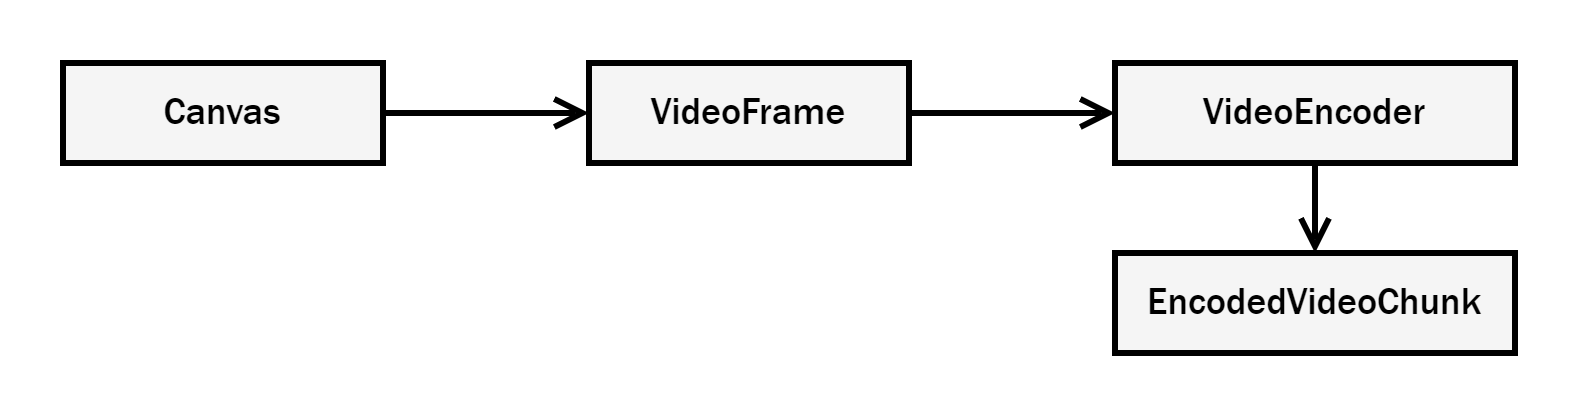
\includegraphics[width=\textwidth]{res/webcodecs.png}
    \caption{The path to encode a video file with WebCodecs, from a \texttt{Canvas} to the encoded chunks.}
    \label{fig:webcodecs_diagram}
\end{figure}

In our implementation, the \texttt{VideoFrame} is constructed from an HTML \texttt{canvas}, which is an element with a predefined size on which an image can be drawn. Once we have the canvas, the \texttt{VideoFrame} is created like this:

\begin{minted}[frame=single]{js}
const frame = new VideoFrame(canvas, {
    timestamp: frag.start,
});
\end{minted}

To encode the frame, we first need to create a \texttt{VideoEncoder} instance specifying a codec configuration supported by the browser. Unfortunately, it is not possible to obtain a list of supported configurations; therefore, a possible strategy is to make multiple attempts until a working configuration is found. The async static method \texttt{VideoEncoder.isConfigSupported(config)} lets developers check whether the input configuration is supported.

The code example in Figure \ref{fig:webcodecs_videoencoder} shows how a \texttt{VideoEncoder} instance can be configured. In this case, the following options are specified:

\begin{itemize}
    \item \textbf{Codec}: a string that defines which codec should be used for encoding.
    \begin{itemize}
        \item The characters before the dot define the name of the codec, as specified by the WebCodecs Codec Registry. For example, in \texttt{avc1.64001f} the string \texttt{avc1} refers to AVC/H.264.\footnote{\url{https://www.w3.org/TR/2022/DRY-webcodecs-codec-registry-20221013/}}
        \item The suffix of the string is specific to the coding format and contains information such as the profile, level, bit depth, etc., that are needed by the decoder. In the case of H.264, the six characters are in hexadecimal format: the first two characters refer to the profile (in the example, \texttt{64} corresponds to \texttt{High}), while the last two declare the level (in the example, \texttt{1f} corresponds to Level 3.1).
    \end{itemize}
    \item \textbf{Width and height}: the resolution of the output video.
    \item \textbf{Bitrate}: the target average bitrate to use for encoding.
    \item \textbf{Framerate}: the number of frames per second of the output video.
    \item \textbf{AVC} contains H.264-specific options. In this case, we are asking the encoder to return a stream in the Annex B format.
\end{itemize}

There are also options to control whether \textbf{hardware acceleration} should be preferred, if available, and whether to \textbf{optimize for low latency}.

\begin{figure}
    \centering
    \begin{minted}[frame=single,linenos]{js}
const codec = 'avc1.64001f';
const width = 1280;
const height = 720;
const birate = 3_000_000;
const framerate = 25;

const config = {
    codec,
    width,
    height,
    bitrate,
    framerate,
    avc: { format: 'annexb' as AvcBitstreamFormat },
};

const encoder = new VideoEncoder(init);
encoder.configure(config);
\end{minted}
    \caption{TypeScript code snippet that initializes and configures and instance of the WebCodecs \texttt{VideoEncoder}.}
    \label{fig:webcodecs_videoencoder}
\end{figure}

Encoding complex video sequences with \texttt{VideoEncoder} requires careful considerations on the rate with which frames should be provided to the encoder, but in our case we just need to encode a single frame, so the implementation is simpler. The encoding of a frame can be started with the following function call:

\begin{minted}[frame=single]{js}
encoder.encode(frame);
\end{minted}

In these code samples, error handling and proper management of the resources lifecycle are omitted for brevity.

When a newly encoded video chunk is available, a callback defined as a property of the \texttt{init} object passed to the \texttt{VideoEncoder} is invoked. All the data required by the decoder, including the SPS and PPS metadata, are included in the provided bitstream in the Annex B format.

As mentioned above, the video frame can be created starting from a 2D \texttt{canvas} that can contain any picture. If we want to create a video segment made of a still picture of the last frame shown on the screen, we can do that with the \texttt{canvas} API. The following code block shows how we can draw the current image rendered by a \texttt{<video>} element on a \texttt{canvas}.

\begin{minted}[frame=single]{js}
const canvas = document.createElement('canvas');
const ctx = canvas.getContext('2d');
ctx.drawImage(video, 0, 0, canvas.width, canvas.height);
\end{minted}

Note that the source image resolution might not correspond to the one of the \texttt{canvas}. For this reason, we must specify the destination dimensions when calling the \texttt{drawImage} function, so that the picture is scaled correctly.

Also, while the filler segment could 
in theory be of any resolution independently from the current ABR level, in our implementation we try to match the expected resolution.

\subsection{Changes to the testbed}
\label{sec:improvements/impl/newtestbed}

In the previous sections, we introduced how an alternative user experience for live streaming can be built, taking advantage of multiple techniques such as giving priority to audio segments, dropping segments and generating filler segments on the fly. To \textbf{test and integrate the solution with the testbed}, we had to make some changes to it.

First, we swapped the \hlsjs{} implementation with our modified version. Since we are building the application with \texttt{Vite}, which bundles the dependencies declared in the \texttt{package.json} file, we can replace the version of the \hlsjs{} library with a local module or the path to a remote repository. In our case, we chose to fork the \texttt{hls.js} repository on GitHub so that \texttt{npm} can pull the modified library from there.

For WebAssembly to work, the initialization code mentioned in Section \ref{sec:improvements/impl/muxing} must be executed on the web page. This initialization code can be included in two ways: through the TypeScript code of the \hlsjs{} library, or directly in the HTML page of the testbed frontend. In the second case, we must modify the testbed to include the WebAssembly initialization.

If audio prioritization is not implemented directly in the modified version of \hlsjs{}, we must modify the \texttt{Hls} instance creation to override the HTTP loader, as seen in Section \ref{sec:improvements/priority}. Finally, for a proper analysis of the performance of the solution it would be useful to know when a segment was dropped and replaced with a filler. To do this, the statistics collector on both the frontend and the backend need to be updated to collect this information.

\section{Experimental results}
\label{sec:improvements/results}

In this section, we analyze some results that we obtained with the modified testbed and observe whether the solution indeed produces a better user experience.

Figure \ref{fig:filler1} shows the buffer health plot for an experiment ran with the modified \hlsjs{} library. The protocol is HTTP/3 so that priorities can be used. The network pattern is \texttt{spike}, the one that in previous sections showed bad performance.

\begin{figure}[h]
    \centering
    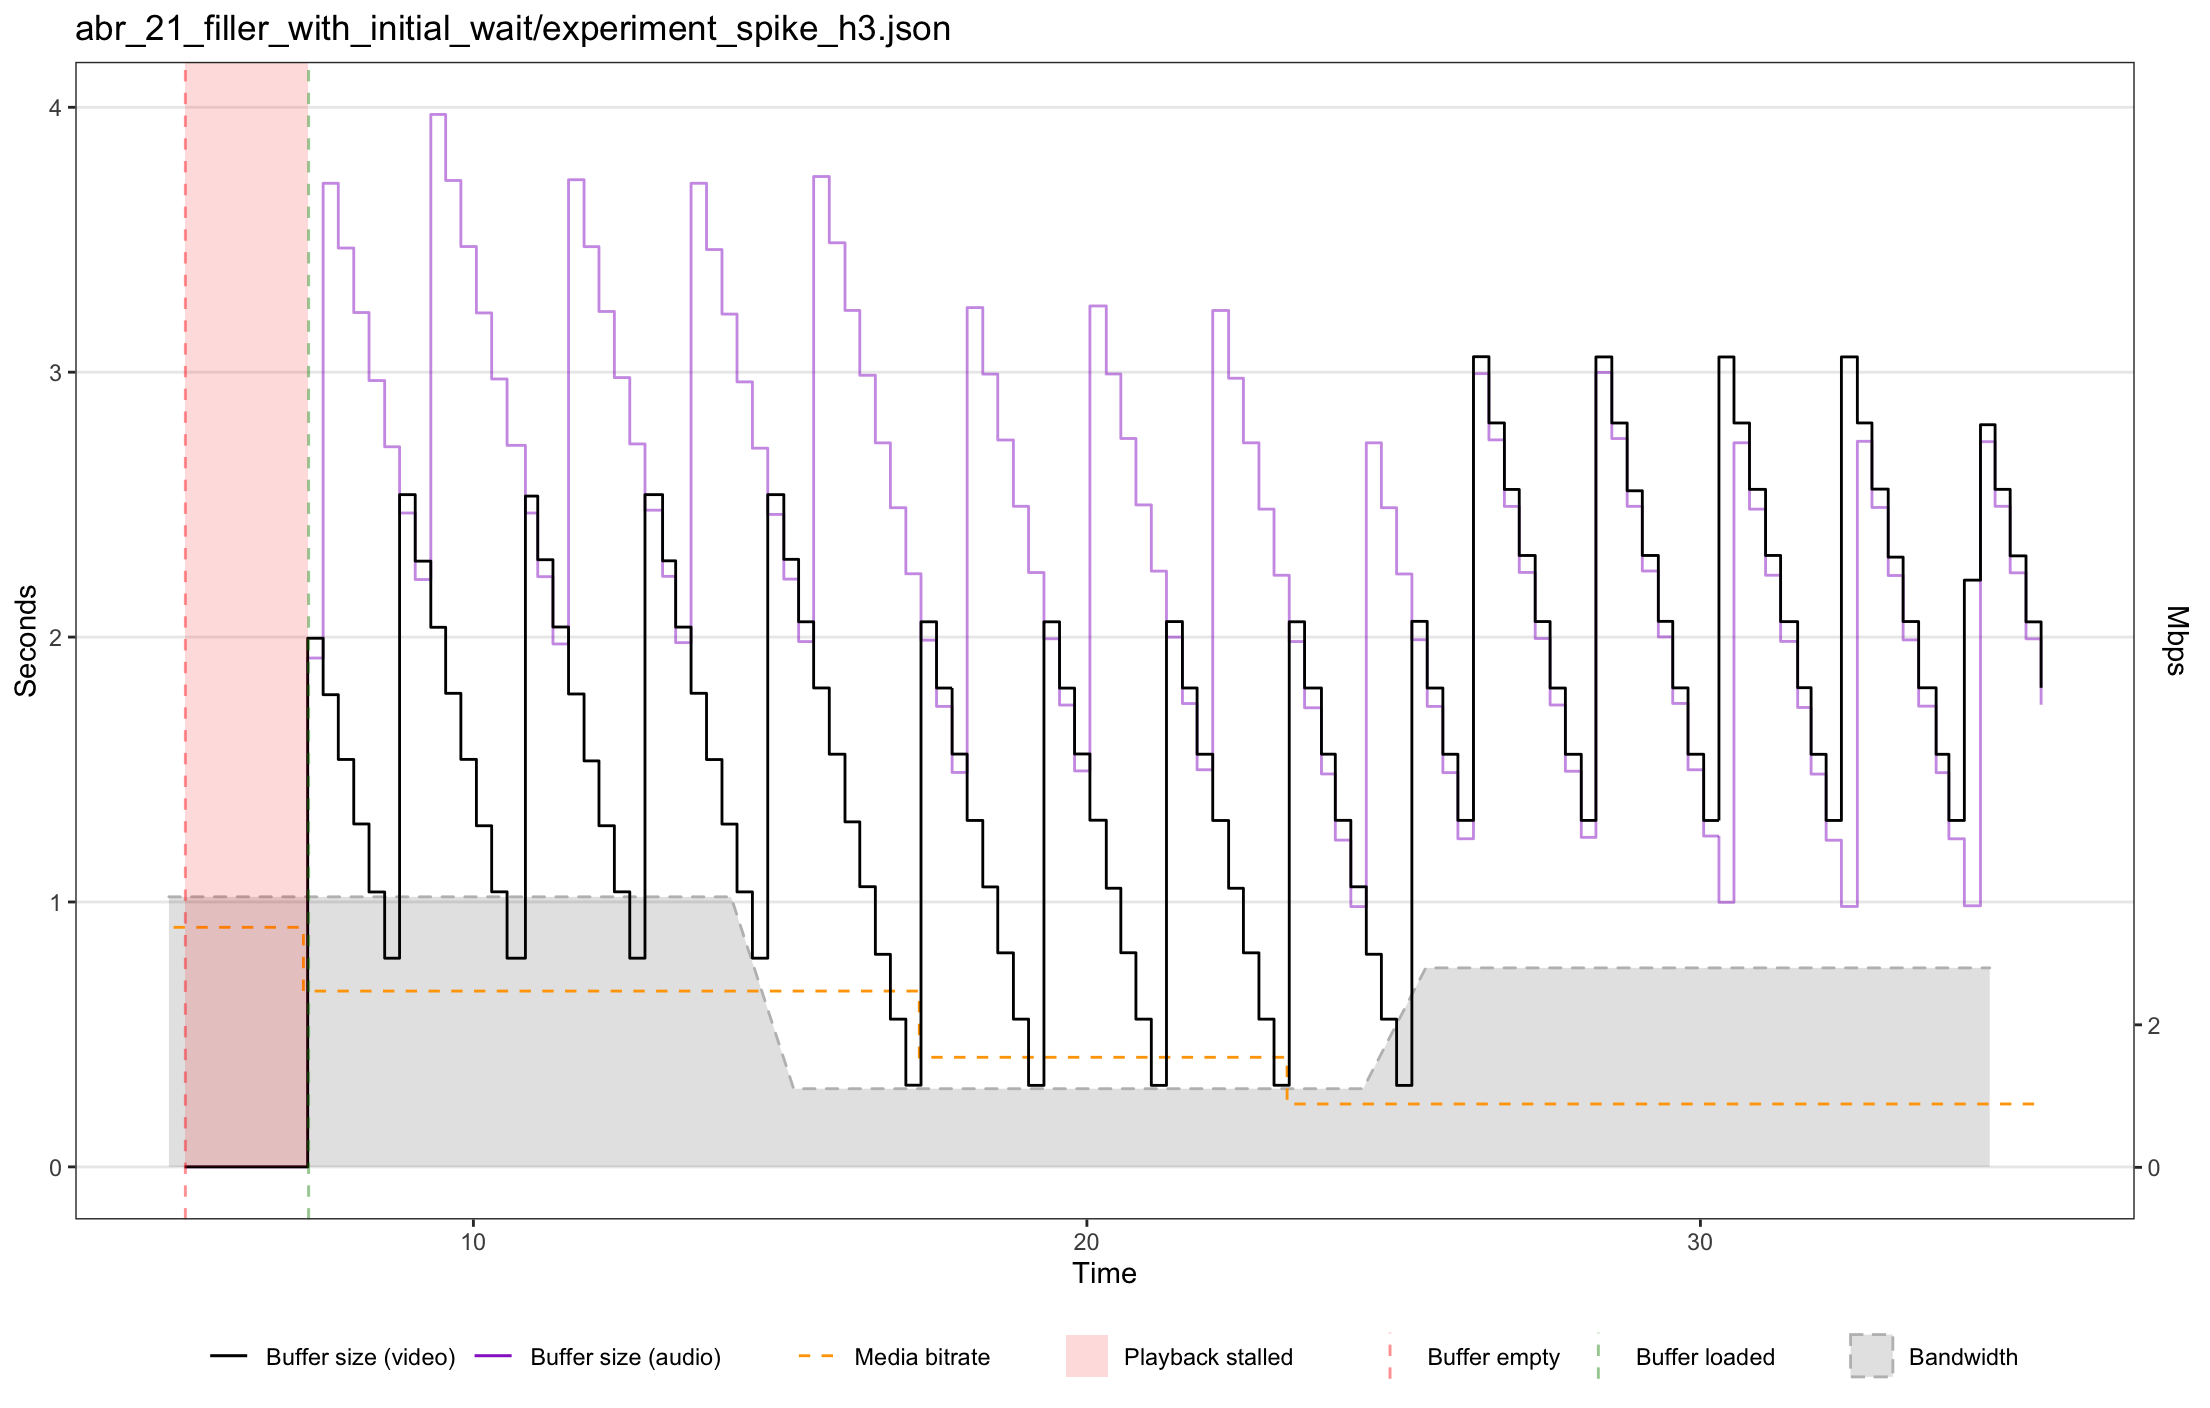
\includegraphics[width=0.9\textwidth]{res/impr_hls_filler.png}
    \caption{Buffer health plot for an experiment using the modified \hlsjs{} library. The protocol is HTTP/3 and priority is given to audio. The network pattern is \texttt{spike}. Outdated segments are dropped and replaced by the filler segment (dark areas).}
    \label{fig:filler1}
\end{figure}

As we can see, \textbf{the playback stalls have been completely removed}. Playback is not interrupted because there is always some audio in the buffer to play. The dark areas refer to the segments that have been dropped and replaced with a filler segment.

In Figure \ref{fig:filler2} we can also see the live latency and the waterfall. It is clear that with this solution the live latency stays stable even during the congestion periods. In the waterfall diagram, we can see which segments are discarded, represented in black.

\begin{figure}[H]
	\centering
	
	\begin{subfigure}[t]{0.5\textwidth}
		\centering
		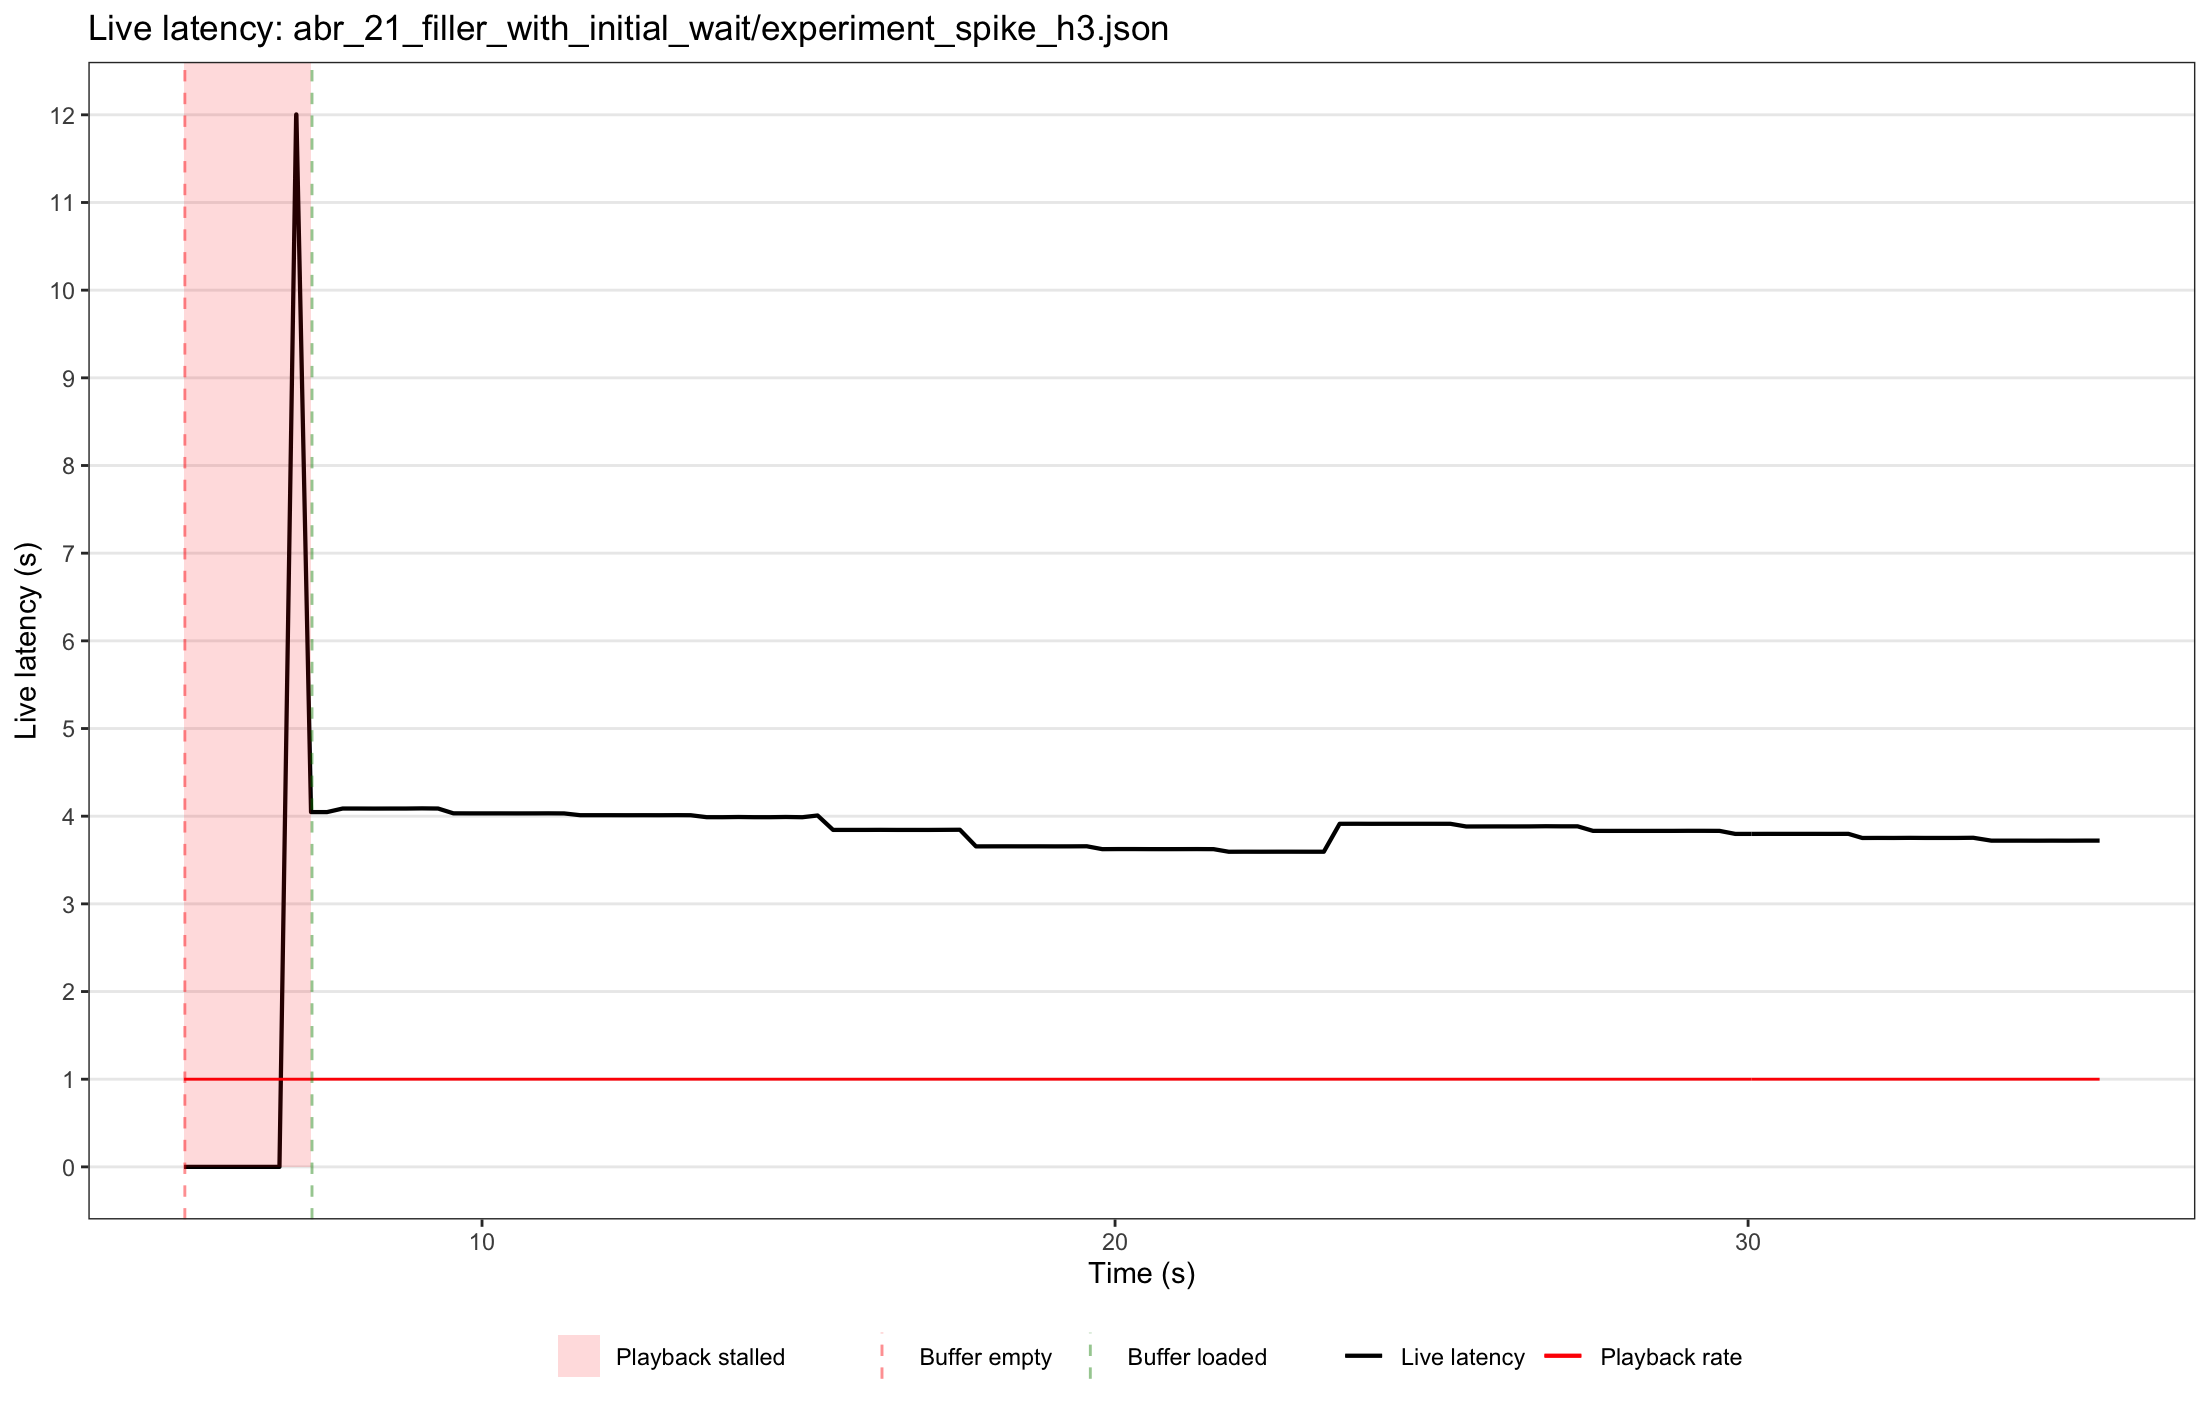
\includegraphics[width=\textwidth]{res/impr_hls_filler_latency.png}
		\caption{Live latency plot.}
		\label{fig:filler2_latency}
	\end{subfigure}%
	~ 
	\begin{subfigure}[t]{0.5\textwidth}
		\centering
		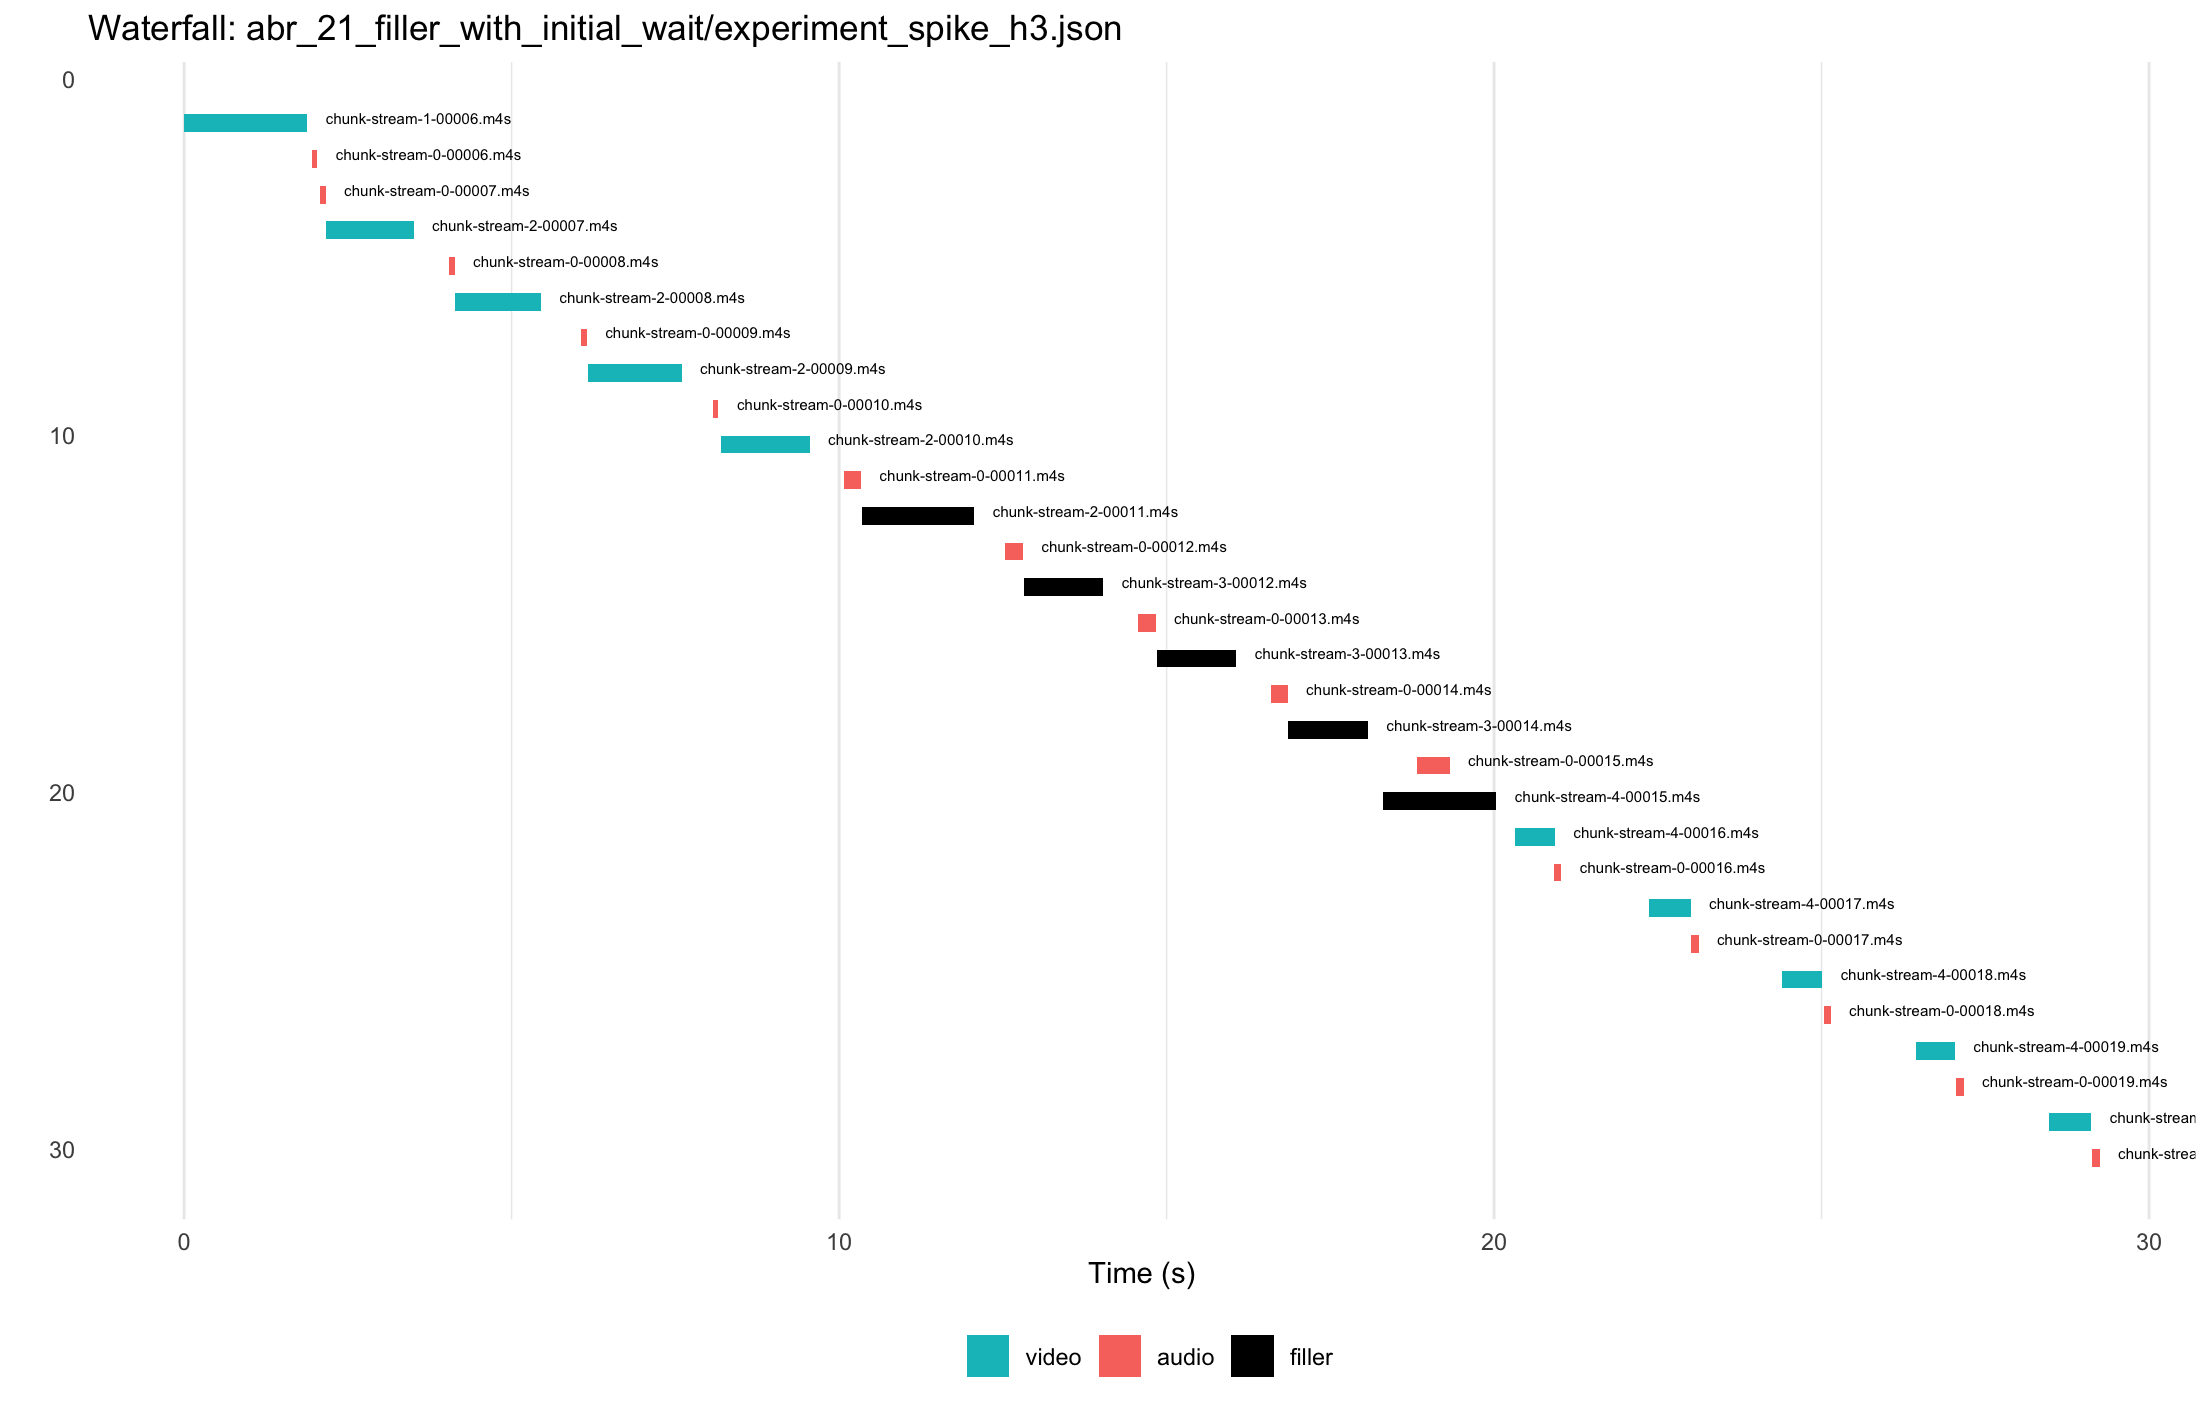
\includegraphics[width=\textwidth]{res/impr_hls_filler_waterfall.png}
		\caption{Waterfall diagram.}
		\label{fig:filler2_waterfall}
	\end{subfigure}
	
	\caption{Additional plots for the experiment with modified \hlsjs{} version over HTTP/3 with the \texttt{spike} network pattern.}
	\label{fig:filler2}
\end{figure}

Note that the bandwidth drop in the \texttt{spike} pattern is quite aggressive and in general shows very low bandwidth, so the fact that five consecutive segments are dropped is somehow expected. As mentioned in previous sections, running the experiment multiple times results in slightly different results. However, there is still room for improvement. For example, the discarding of the segment should free up the bandwidth needed for loading the next segment, but we see that this is not the case with this particular configuration. In the final chapter, we will propose some ideas that might be worth investigating in the future to further improve the solution.


